\chapter{A digit made by the Sun --- I}
\label{sec:digito-solar-i}

\lettrine[ante=\raisebox{-1.5ex}{\large ---},lines=2]{E}{ach of the} digits that will indicate the time will be for sun rays ---Antonia started, offering to Cecilia figure~\ref{fig:digitos}.


\begin{figure}[ht]
  \centering
\centerline{
  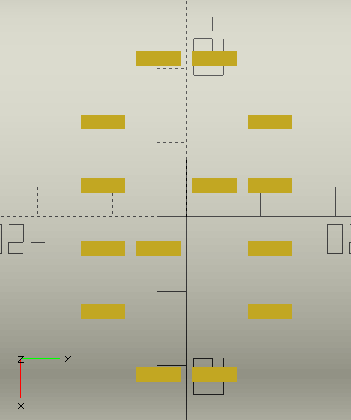
\includegraphics[height=.25\textwidth]{imagenes/cero}
  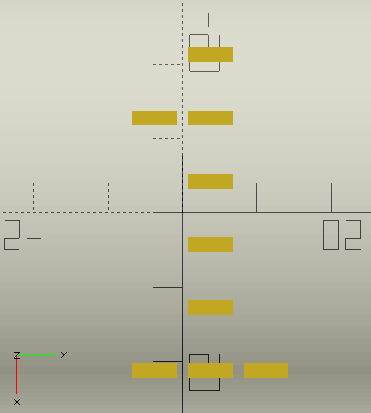
\includegraphics[height=.25\textwidth]{imagenes/uno}
  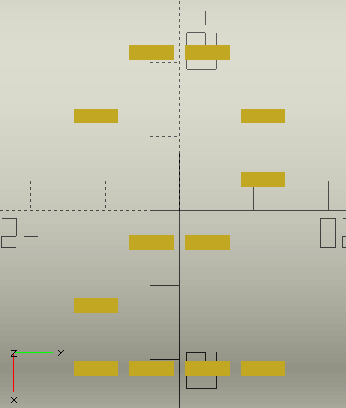
\includegraphics[height=.25\textwidth]{imagenes/dos}
}
\centerline{
  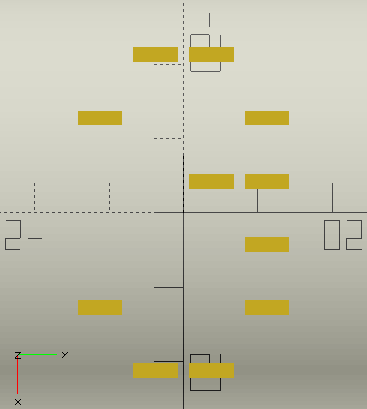
\includegraphics[height=.25\textwidth]{imagenes/tres}
  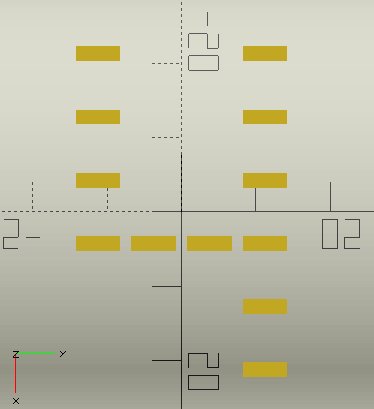
\includegraphics[height=.25\textwidth]{imagenes/cuatro}
  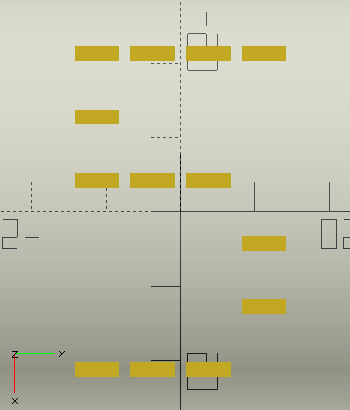
\includegraphics[height=.25\textwidth]{imagenes/cinco}
}
\centerline{
  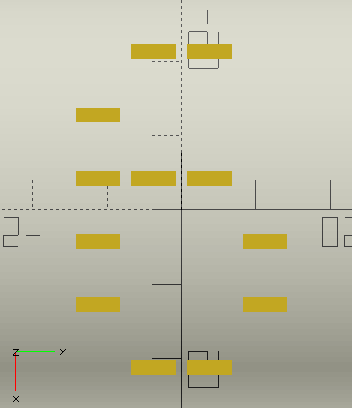
\includegraphics[height=.25\textwidth]{imagenes/seis}
  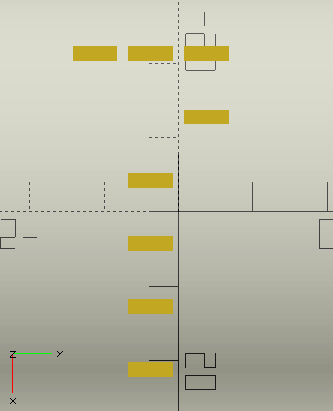
\includegraphics[height=.25\textwidth]{imagenes/siete}
  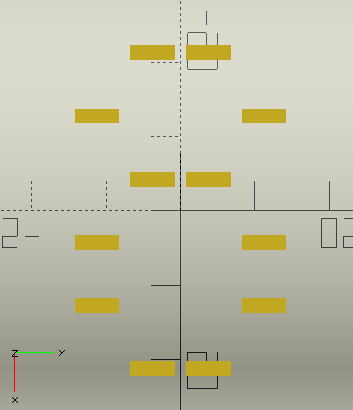
\includegraphics[height=.25\textwidth]{imagenes/ocho}
  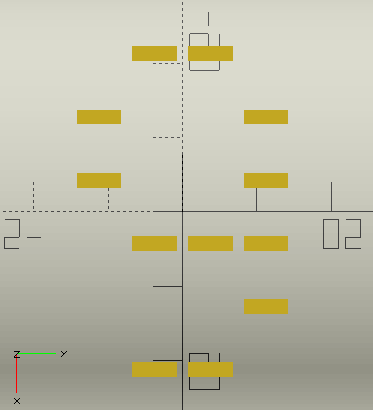
\includegraphics[height=.25\textwidth]{imagenes/nueve}
}  
  \caption{Digits made of sunbeams.}
  \label{fig:digitos}
\end{figure}

---What good designs! Did you make them? Cecilia asked.

   ``No,'' Antonia agreed without difficulty. I unscrupulously copied the visual arrangement from the model that inspired me in general \url{https://www.thingiverse.com/thing:1068443}.

---Ah!\
You're a catch... ---Cecilia smiled mischievously.

---It was only the visual aspect ---Antonia took refuge in a defensive attitude. The logic and the text I reconstructed myself.

   Cecilia looked at her friend carefully for a few moments; I didn't know whether to ask him a question. Finally he released her: ---Antonia... Why did you redo a model that was already solved? by other person? Wasn't it enough to download and print it?

Antonia returned Cecilia's gaze: ---Why are you doing this course? he replied. Why did you get to page~\thepage{} of this little manual?

   The two friends looked at each other in silence. Cecilia understood that few things were compared to solving, by oneself, a difficult problem and with a beautiful-looking end result. And the digital Sundial combined both qualities perfectly.

``As you may have noticed,'' Antonia resumed, ``all the digits are based on the same pattern of six rows and four columns of pixels. The difference between the digits lies in which pixels are 'on' or 'off'; although it would be better to say 'open' or 'closed', since each represents a hole in the semi-cylinder of the clock.

``The '1' seems to have only three columns,'' Cecilia observed.

   ``The fourth column is here, only it's made up of 'closed two' pixels,'' Antonia clarified. Cecilia thought it was a bit artificial. ``And why not think, then, that it is made up of 17
rows and 48 columns, most of them 'closed'?'' he thought, but let her continue.

\begin{figure}[t]
  \centering
  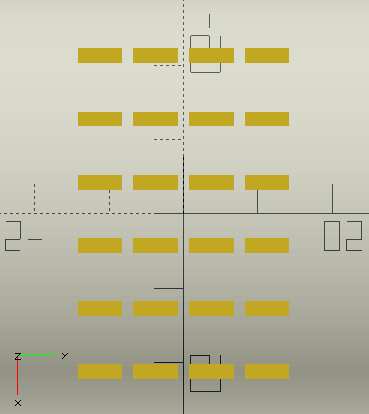
\includegraphics[width=.35\textwidth]{imagenes/matriz.png}
  \caption{Matrix of pixels that will form each digit.}
  \label{fig:matriz}
\end{figure}

\begin{figure}[ht]
  \centering
  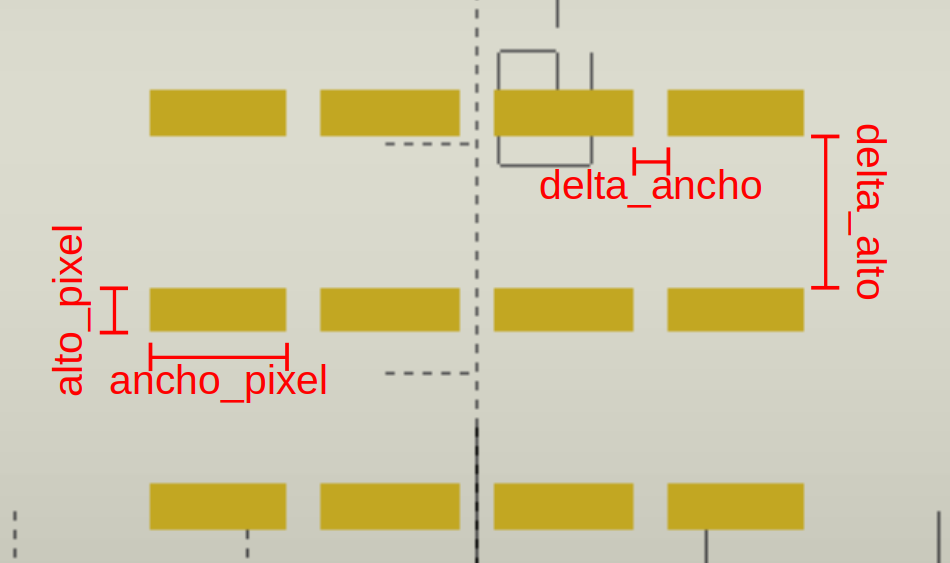
\includegraphics[width=.55\textwidth]{imagenes/matriz-anotada-2}
  \caption{Antonia writes down the matrix in order to locate each pixel.}
  \label{fig:matriz-anotada-2}
\end{figure}
  

---To clarify ideas, we are going to see all the rays 'on'---said Antonia, pointing to the figure~\ref{fig:matriz}, while she continued with the slow tone that foreshadowed one of her long explanations
---. Each digit, then, will be formed by leaving the appropriate pixels open or closed. But before we see how to choose each one, I think we better solve the problem of placing each ray in a neat and orderly arrangement of rows and columns.

Cecilia made an intelligent face: 

---Shall we use the transformation \lstinline!translate!? 

---Yes, it's  better; but the question is how? Antonia seemed not to have caught the irony. It helps me to start making drawings on top ---he added, making the figure~\ref{fig:matriz-anotada-2}.

\guillemotright In order to correctly distribute the pixels, we must agree not only on the size of each pixel (expressed in our acquaintances \texttt{ancho\_pixel} and \texttt{alto\_pixel}) but also on the separation between pixels: it occurred to me to call them  \texttt{delta\_ancho} and \texttt{delta\_alto}.

Cecilia had no objection.

---Now we have to be able to distinguish each pixel from the others. Give them a 'name', let's say. It occurred to me to do it in reference to the row and column they occupy in the array, it can't be the worst
way ---said Antonia.

\begin{figure}[ht]
  \centering
  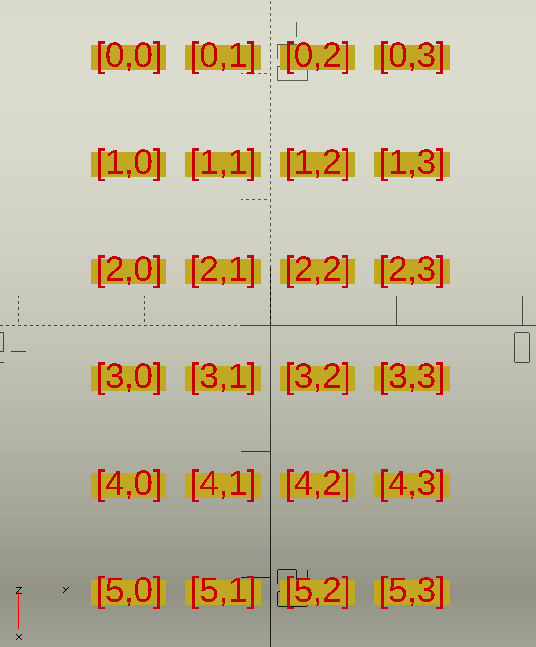
\includegraphics[width=.45\textwidth]{imagenes/matriz-anotada-coordenadas}
  \caption{Antonia names each pixel with the integer coordinates of its matrix.}
  \label{fig:matriz-anotada-coordenadas}
\end{figure}
  
\guillemotright{}Thus, the first pixel will be the one in row 0 and column 0, etc. As we commented in the chapter~\ref{sec:vectores}, it is usual to refer to the positions within a rectangular array starting with 0 ---remembered Antonia, and continued?: Now, the most difficult thing: locate the position in \coord{X} and \coord{Y} of each pixel knowing its row and column, taking
into account the values of \texttt{ancho\_pixel}, \texttt{alto\_pixel}, \texttt{delta\_ancho} and
\texttt{delta\_alto}.

\guillemotright{}To go step by step, it seems better to locate the center of the
pixel as the origin of the coordinates \texttt{[0,0]}. Yes, I know ---he went ahead
---; we want the center of the arrangement to be the one at the origin of coordinates; but I think it's easier to start thinking about it that way.

Cecilia didn't feel like contradicting Antonia, basically because she still didn't know exactly where she was going on that road that already seemed too long to her.

---Very well, Cacilia; I've already talked a lot--- Antonia looked at her friend with her eyes barely closed and with a shine that, once again, seemed like a plea. Now we should be able to calculate the value of de \coord{X} and \coord{Y} for any pixel: say, for example, the  \texttt{[3,2]}.

\begin{figure}[ht]
  \centering
  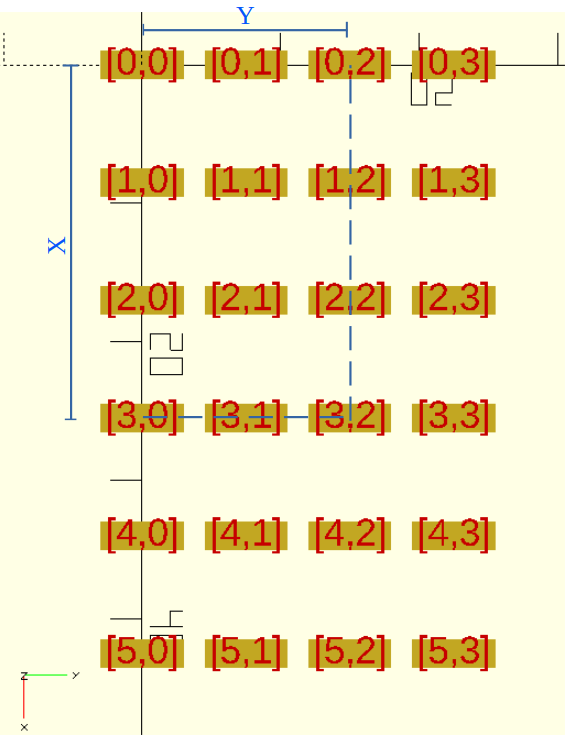
\includegraphics[width=.42\textwidth]{imagenes/matriz-coordenadas-1}
  \caption{Antonia challenges Cecilia to find the coordinates
\coord{X} \coord{Y} of each pixel; in particular, of \texttt{[3,2]}.}
  \label{fig:matriz-coordenadas-1}
\end{figure}

Antonia was silent, and Cecilia knew that that plural was, like other times, very singular.

``Will you let me do some drawings?'' Cecilia asked as she took the keyboard for herself.

\begin{figure}[ht]
  \centering
  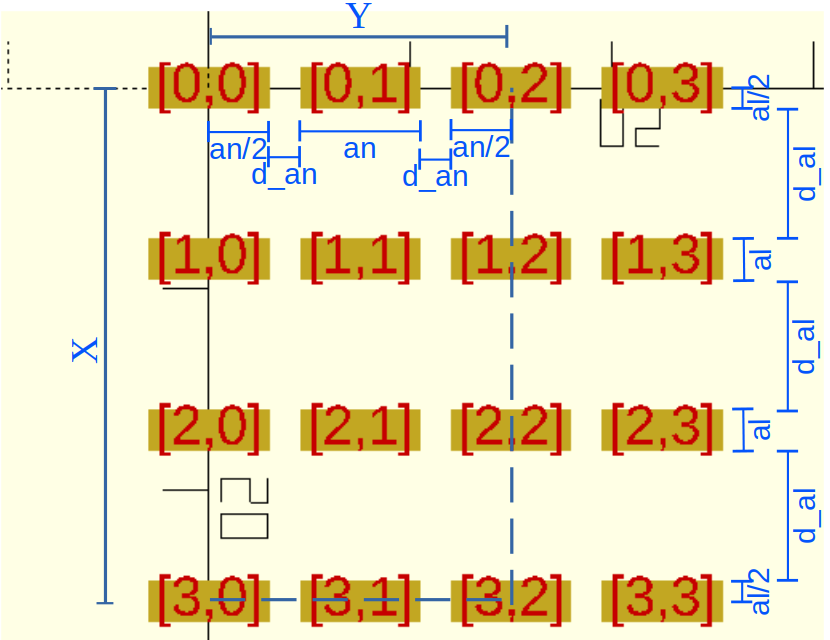
\includegraphics[width=.6\textwidth]{imagenes/matriz-coordenadas-4.png}
  \caption{Cecilia tries to express the coord{X} \coord{Y}  coordinates of
each pixel, starting with \texttt{[3,2]}.}
  \label{fig:matriz-coordenadas-4}
\end{figure}

---------------------------------------------------------------------

\guillemotright ¡Uf! Me costó... ---reconoció mientras se reclinaba
pesadamente contra el respaldo de la silla y contemplaba la flamante
figura \ref{fig:matriz-coordenadas-4}---. Como no me entraba en el
dibujo, tuve que usar abreviaturas: \texttt{an} es
\texttt{ancho\_pixel}, \texttt{d\_an} es \texttt{delta\_ancho}... en
fin, creo que lo demás se entiende.

Antonia asintió con entusiasmo.

---Por lo que veo ---Cecilia continuó---, la coordenada \coord{Y} del
pixel \texttt{[3,2]} es igual a
$\frac{\text{an}}{2}+\text{d\_an}+\text{an}+\text{d\_an}+\frac{\text{an}}{2}=2\times
\text{an} + 2\times\text{d\_an}=2\times(\text{an}+\text{d\_an})$. Por
otra parte, la coordenada \coord{X} parece ser igual a... ---Cecilia
masculló apenas los pasos intermedios---:
$3\times(\text{al}+\text{d\_al})$.

Antonia, con una amplia sonrisa de satusfacción, tomó la palabra y el
teclado:

---Pasemos en limpio, entonces:

\[
  \text{Para el pixel }[3,2]: \left\{
    \begin{aligned}
      X&=3\times(\text{al}+\text{d\_al})\\
      Y&=2\times(\text{an}+\text{d\_an})
    \end{aligned}
  \right.
\]

Cecilia contemplaba las ecuaciones y el grafico. No pasó mucho tiempo
hasta que encontró el patrón subyacente:

---¡Claro! ---exclamó exultante---. La coordenada \coord{X} del pixel
\texttt{[i,j]} es $i$ veces $(\text{al}+\text{d\_al})$ , mientras que
la coordenada \coord{Y}, análogamente, es $j$ veces
$(\text{an}+\text{d\_an})$.\footnote{Sería bueno demostrar
  fehacientemente un aserto tan general (Nota del
  Editor).}$^,$\footnote{¿No tenés nada mejor que hacer?  (Nota de
  Cecilia, Antonia y Luis).}

Antonia confirmó la conclusión de Cecilia con indisimulada alegría:

---Vamos a dejarlo bien patente ---propuso.


\begin{equation}
  \text{Para el pixel }[i,j]: \left\{
    \begin{aligned}
      X&=i\times(\text{al}+\text{d\_al})\\
      Y&=j\times(\text{an}+\text{d\_an})
    \end{aligned}
  \right.\label{eq:coordenadas-matriz}
\end{equation}

\guillemotright Creo que es hora de darle a tantas vueltas y rodeos la
forma de un texto para \openscad{}, ¿no te parece? ---invitó Antonia,
cediéndole el teclado con gesto ceremonioso.

Cecilia lo tomó con decisión, aún no del todo segura de lo que iba a
escribir, pero con entusiasmo y la confianza de que las teclas
\keystroke{Supr} y \keystroke{$\Longleftarrow$} le serían fieles. Tras
mucho escribir, borrar y consultar con las ecuaciones, obtuvo lo
siguiente:

%    \begin{center}
 % \begin{minipage}[]{1\textwidth}%\vspace{0pt}
    \begin{lstlisting}
alto_pixel  = 2;
ancho_pixel = 6;      
delta_alto  = 6.5;
delta_ancho = 1.5;

module digito(alfa){
  for(i=[0:5],j=[0:3]){
   x=i*(alto_pixel+delta_alto);
   y=j*(ancho_pixel+delta_ancho);
   translate([x,y,0])
    rayo_de_sol(alfa);
  }
}

digito(alfa=90);
    \end{lstlisting}
%  \end{minipage}\hfill

    \begin{figure}[ht]
      \centering
    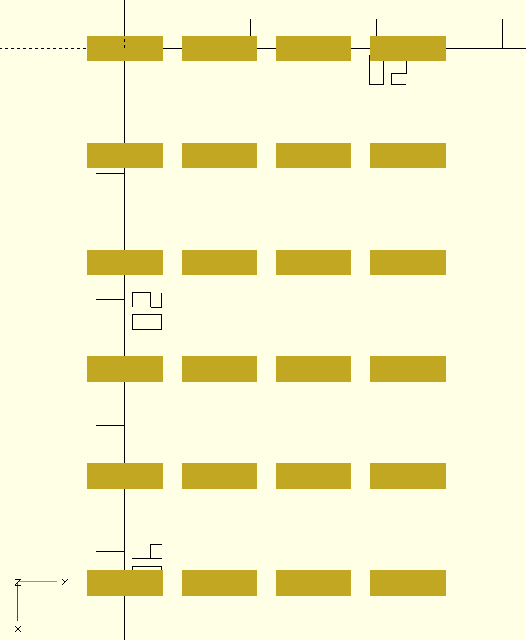
\includegraphics[width=.4\textwidth]{imagenes/matriz-completa}  
    \caption{Cecilia manages to produce a complete array of lit pixels.}
      \label{fig:matriz-completa}
    \end{figure}
    



    Cecilia se sentía tan feliz contemplando el resultado plasmado en
    la figura \ref{fig:matriz-completa} que pensaba que podría releer
    su texto hasta que el Sol se
    apagara. % Sabía que el objetivo del presente
    % capítulo era encontrar una manera de crear una ordenación
    % rectangular de pixeles, para luego elegir cuales abrir y cuales
    % cerrar; por esa razón, no puso mucho cuidado a la hora de nombrar
    % su módulo: \texttt{arreglo\_completo} era suficientemente bueno
    % para un módulo auxiliar, que sería borrado tras comprobarse la
    % efectividad del método.

    Dentro del módulo creaba un doble bucle: las variables \texttt{i}
    y \texttt{j} recorrían los valores de 0 a 5 y de 0 a 3,
    respectivamente, a fin de abarcar todas las filas y columnas.

    Luego, en las líneas 8 y 9 calculaba las coordenadas \coord{X} e
    \coord{Y} de cada pixel, aplicando las ecuaciones
    \ref{eq:coordenadas-matriz}.

    Por último, en las líneas 10 y 11 creaba para cada pixel un rayo
    de Sol trasladado a las coordenadas recién calculadas.

    ---Parece mentira que además funcione, ¿no? ---Antonia interrumpió
    los pensamientos de Cecilia---. A mí me pasa lo mismo: una cosa es
    \emph{saber} que un algoritmo debe funcionar, y otra muy distinta
    es \emph{comprobar} que efectivamente funciona. Es... hermoso.

    Cecilia estaba de acuerdo de todo corazón. Pero Antonia se
    reservaba una objeción:

    ---Fijate la posición del arreglo completo: te quedó centrado en
    su pixel \texttt{[0,0]}, no en su centro.
    
    Cecilia se mordió el labio inferior; la ansiada versión final del
    texto siempre parecía alejarse un poco más.

    ---Es cierto --admitió---; pero parece sencillo de resolver: no
    hay más que trasladar todo una cierta distancia en \coord{X} e
    \coord{Y}... a ver... ---y Cecilia, en breves instantes, pudo
    ofrecer su nueva solución:

    \begin{lstlisting}
module digito(alfa){
  translate([-2.5*(alto_pixel+delta_alto),
             -1.5*(ancho_pixel+delta_ancho),
             0])
   for(i=[0:5],j=[0:3]){
    x=i*(alto_pixel+delta_alto);
    y=j*(ancho_pixel+delta_ancho);
    translate([x,y,0])
     rayo_de_sol(alfa);
   } 
}

digito(alfa=90);
    \end{lstlisting}

  
  \begin{figure}[ht]
    \centering
    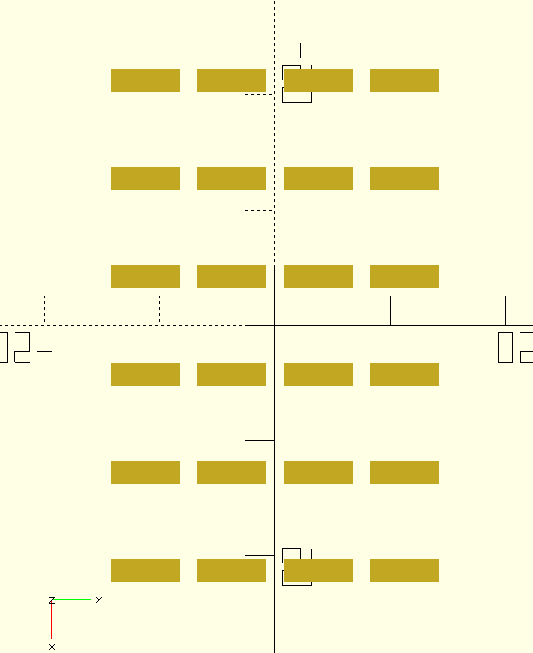
\includegraphics[width=.45\textwidth]{imagenes/matriz-completa-centrada-0}    
    \caption{Cecilia properly centers the array at the origin of coordinates.}
    \label{fig:matriz-completa-centrada-0}
  \end{figure}
  


    Antonia aprobó la modificación con una sonrisa y un aplauso
    apagado: la traslación del arreglo ocurría gracias al
    \lstinline!translate! de las líneas 2 a 4, que afectaba a todo lo
    creado por el \lstinline!for! inmediato siguiente.

    Pero ahora fue Cecilia quien parecía mirar su propio texto con
    ojos críticos: las líneas 2 y 3 le parecieron demasiado similares
    a las 6 y 7. <<¿No estoy trasladando dos veces, y con una lógica
    similar, los mismos rayos de Sol?>> ---pensó---. <<¿Por qué no
    hacerlo de una sola vez..?>>. Y se lanzó a plasmar su idea:

\begin{lstlisting}
module digito(alfa){
  for(i=[0:5],j=[0:3]){
   x=(i-2.5)*(alto_pixel+delta_alto);
   y=(j-1.5)*(ancho_pixel+delta_ancho);
   translate([x,y,0])
    rayo_de_sol(alfa);
  } 
} 

digito(alfa=90);
    \end{lstlisting}


    % \begin{figure}[ht]
    %   \centering
    %   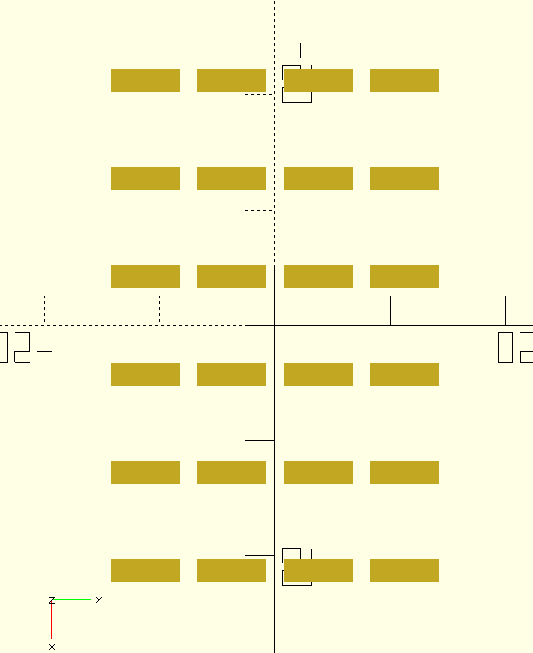
\includegraphics[width=.36\textwidth]{imagenes/matriz-completa-centrada-0}
    %   \caption{Cecilia pule su texto, transformando dos pares de
    %     traslaciones en uno solo.}
    %   \label{fig:matriz-completa-centrada-0-2}
    % \end{figure}


    
    ---Brillante, Cecilia, brillante...  ---Antonia quizá exageraba,
    pero a Cecilia no le importó: estaba muy orgullosa de su
    texto---. Esencialmente, sacaste factor común a las ecuaciones de
    las dos traslaciones.  Después de todo,
    $-2.5 \times (\text{alto\_pixel}+\text{delta\_alto})\, + \, i\times
    (\text{alto\_pixel}+\text{delta\_alto}) = (i-2.5) \times
    (\text{alto\_pixel}+\text{delta\_alto})$, y lo mismo vale para
    \coord{Y}.


    Cecilia creyó que ya podían dar por finalizado el capítulo, pero
    Antonia parecía querer alargarlo un poco más:

    ---Nos queda un detalle, que es mejor que resolvamos ahora. Como
    recordarás del capítulo \ref{semicilindro-1}, cuando restás un
    objeto de otro es conveniente que no compartan una cara en común,
    a fin de evitar una ambigüedad con respecto a la pertenencia o no
    de esa cara al objeto final. Y resulta que tus rayos de Sol se
    apoyan sobre el plano \coord{XY}, al igual que el semicilindro que
    deberán horadar:


\begin{lstlisting}
difference(){
  rotate([-90,0,0])
    semicilindro(150,30,center=true);  
  digito(alfa=90);
}
    \end{lstlisting}
%  \end{minipage}\hfill

    \begin{figure}[ht]
      \centering
      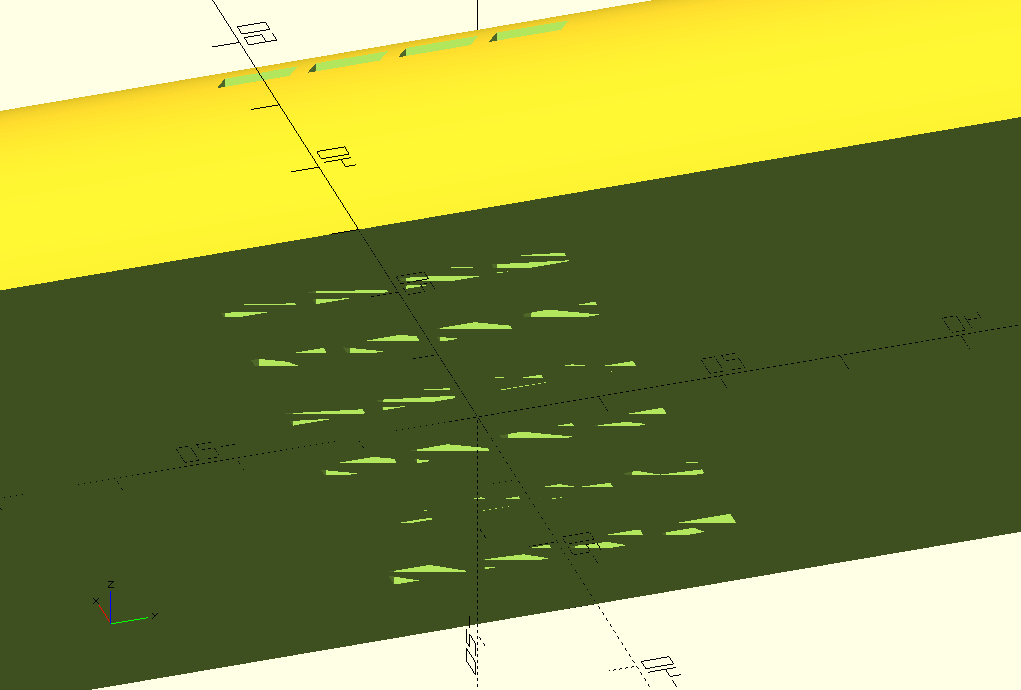
\includegraphics[width=.65\textwidth]{imagenes/digito-al-ras}
      \caption{Antonia shows a subtle bug in the recently conquered Sunbeam.}
      \label{fig:digito-al-ras}
    \end{figure}
     



    ---Noooo.... ---gimió Cecilia, cubriendo sus ojos con una mano. La
    programación comenzó a dejar de parecerle divertida.

    ---Pero Cecilia... ¡no te vas a acorbardar por tan poco!
    ---Antonia la animó sin mucho tacto---. La hacemos fácil: bajamos
    cada rayo un toque. Muy poquito; apenas como para que la
    matemática de las diferencias de \openscad{} no se rompa:

    
\begin{lstlisting}
module digito(alfa){
  for(i=[0:5],j=[0:3]){
   x=(i-2.5)*(alto_pixel+delta_alto);
   y=(j-1.5)*(ancho_pixel+delta_ancho);
   translate([x,y,-0.01])
    rayo_de_sol(alfa);
  } 
}

difference(){
  rotate([-90,0,0])
    semicilindro(150,30,center=true);  
  digito(alfa=90);
}
    \end{lstlisting}
%  \end{minipage}\hfill

    \begin{figure}[ht]
      \centering
      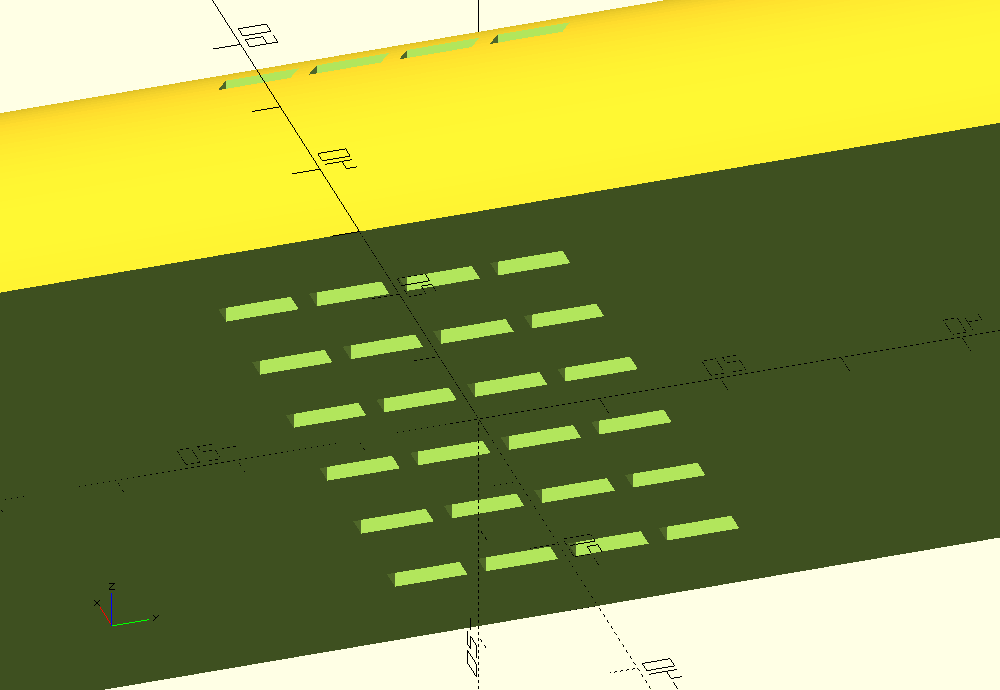
\includegraphics[width=.65\textwidth]{imagenes/digito-apenas-descendido}
      \caption{Antonia solves the bug with a simple but effective expedient.}
      \label{fig:digito-apenas-descendido}
    \end{figure}
      



    ---¿Ves? ---Antonia procuró parecer despreocupada, aunque tal vez
    sobreactuando un poco---. No se trata más que de trasladar cada
    rayo, en la línea 5, -0,01mm en el eje \coord{Z}...

    Cecilia podía apreciar en la figura
    \ref{fig:digito-apenas-descendido} que la solución de Antonia
    funcionaba, pero no estaba muy convencida:
    
    ---¿Y por qué 0,01?

    ---Pues... con que se trate de un valor negativo alcanza, y 0,01
    es mucho más bajo que la resolución de nuestra impresora 3D: en lo
    que respecta al objeto que produciremos, la diferencia con 0 es
    meramente formal ---Antonia trató de que su tono confiado
    pareciera un argumento. Cecilia juzgó que se trataba de una
    solución chapucera, pero no podía negar que funcionaba. Y la
    verdad es que ya estaba cansada.
    
    Pero antes de terminar quiso comprobar que nada se rompía usando
    otros ángulos, como 60º y 150º.



  \begin{figure}[ht]
    \centering
  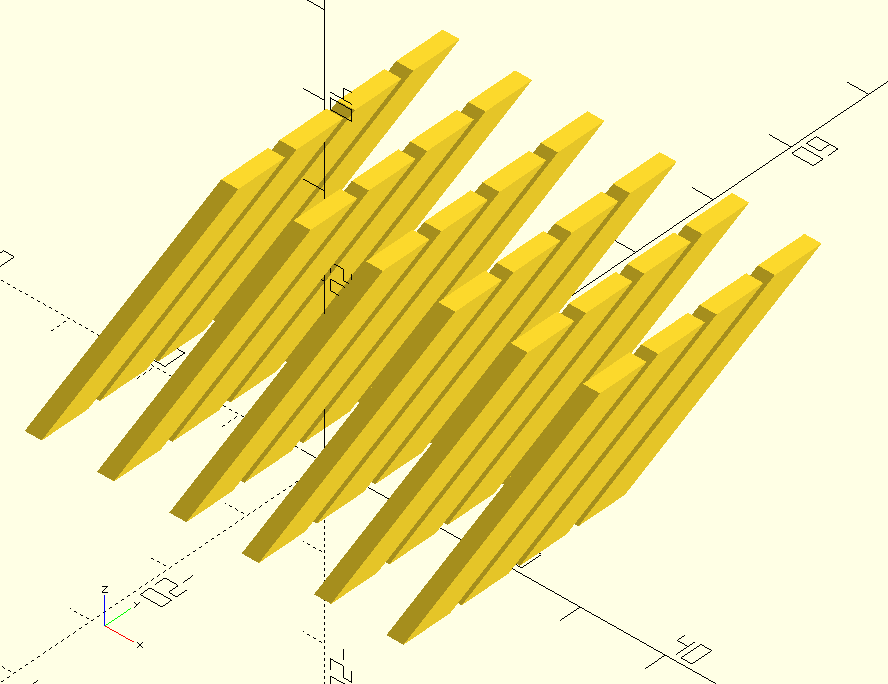
\includegraphics[width=.49\textwidth]{imagenes/matriz-60}\hfill
  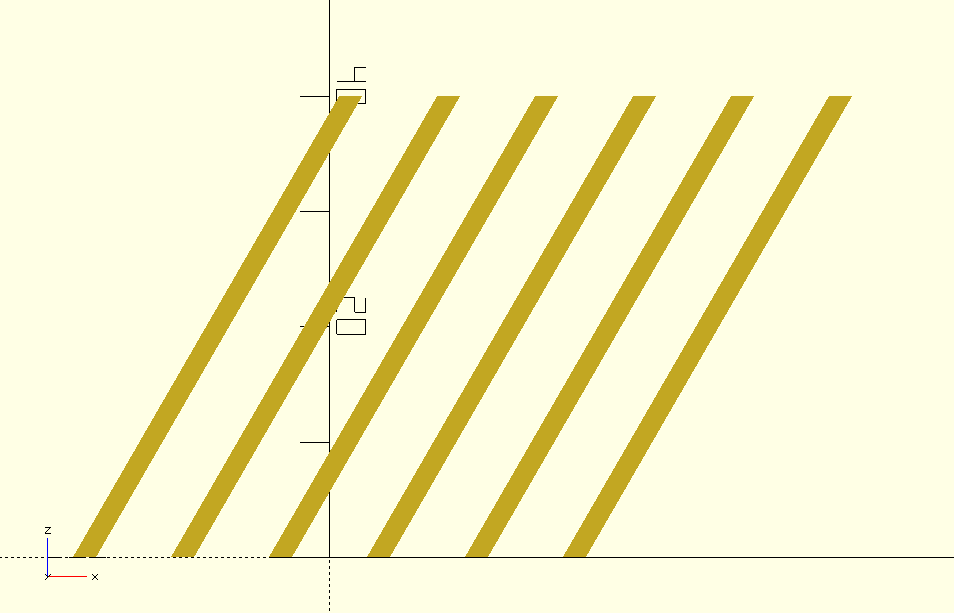
\includegraphics[width=.49\textwidth]{imagenes/matriz-60-perfil}
  \caption{Cecilia checks that the sunbeam works with 60\si{\degree}:
\lstinline!digito(alfa=60);!}
    \label{fig:matriz-60}
  \end{figure}
  

    \begin{figure}[h!]
    \centering
  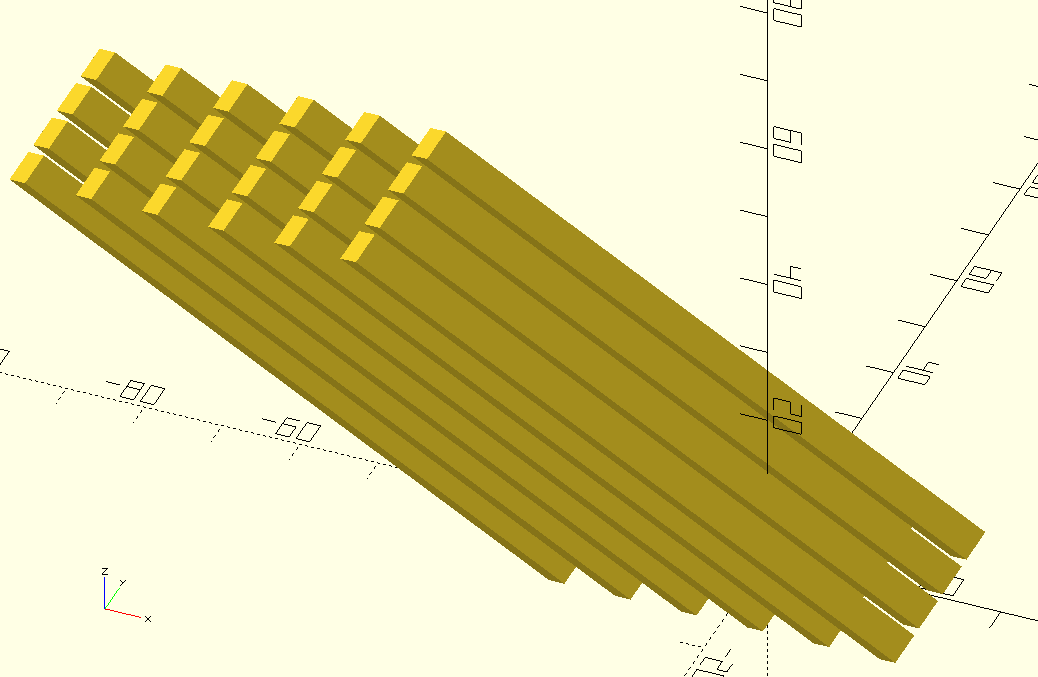
\includegraphics[width=.49\textwidth]{imagenes/matriz-150}\hfill
  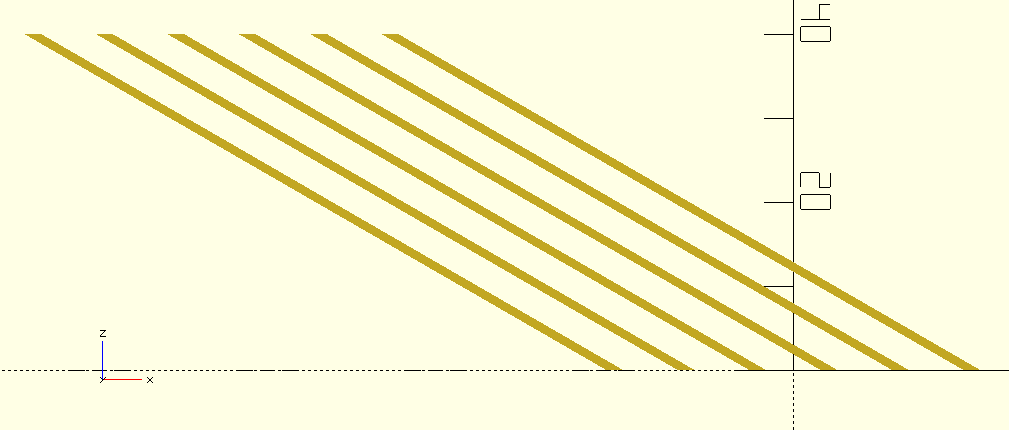
\includegraphics[width=.49\textwidth]{imagenes/matriz-150-perfil} 
    \caption{and with 150\si{\degree}: \lstinline!digito(alfa=150);!}%\vspace{128in}
    \label{fig:matriz-150}
  \end{figure}

It seemed not.




%%% Local Variables:
%%% mode: latex
%%% TeX-master: "../libro"
%%% End:
